\documentclass[a4paper]{article}

\usepackage[top=35mm,bottom=35mm,left=25mm,right=25mm]{geometry}

% Graphics and images
\RequirePackage{graphicx}
\RequirePackage{tikz}
\RequirePackage{tikz-qtree}
\usetikzlibrary{automata, positioning, arrows}

\begin{document}

\subsection{Exercise 3}
\subsubsection{Item a}
\begin{center}
    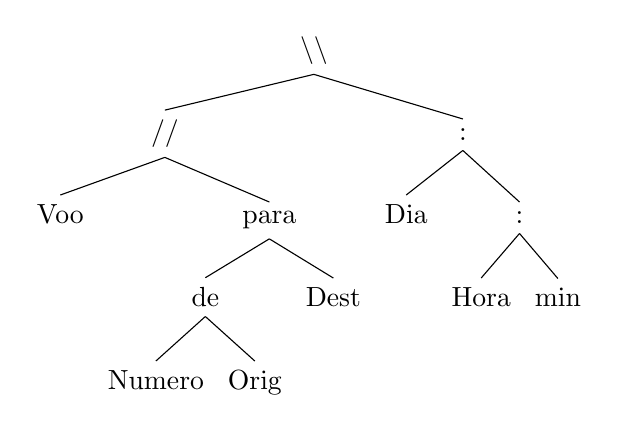
\begin{tikzpicture}
          \Tree 	[.{\textbackslash\textbackslash}
                        [.{//}
                            [.{Voo}
                            ]
                            [.{para}
                                [.{de}
                                    [.{Numero}
                                    ]
                                    [.{Orig}
                                    ]
                                ]
                                [.{Dest}
                                ]
                            ]
                        ]
                        [.{:}
                            [.{Dia}
                            ]
                            [.{:}
                                [.{Hora}
                                ]
                                [.{min}
                                ]
                            ]
                        ]
                    ]
    \end{tikzpicture}
\end{center}

\subsubsection{Item b}
\begin{center}
    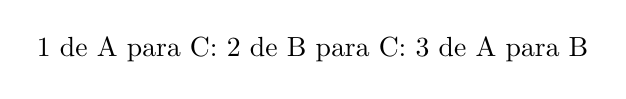
\begin{tikzpicture}
          \Tree 	[.{1 de A para C: 2 de B para C: 3 de A para B}
                    ]
    \end{tikzpicture}
\end{center}
\begin{center}
    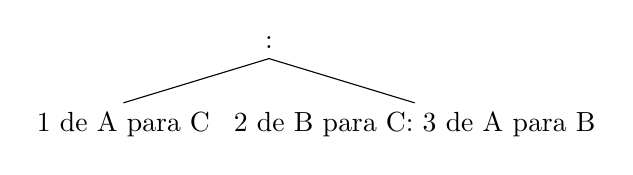
\begin{tikzpicture}
          \Tree 	[.{:}
                        [.{1 de A para C}
                        ]
                        [.{2 de B para C: 3 de A para B}
                        ]
                    ]
    \end{tikzpicture}
\end{center}
\begin{center}
    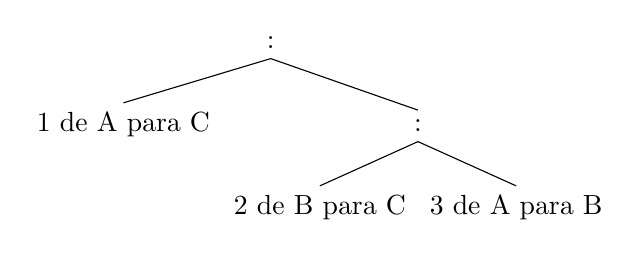
\begin{tikzpicture}
          \Tree 	[.{:}
                        [.{1 de A para C}
                        ]
                        [.{:}
                            [.{2 de B para C}
                            ]
                            [.{3 de A para B}
                            ]
                        ]
                    ]
    \end{tikzpicture}
\end{center}
\begin{center}
    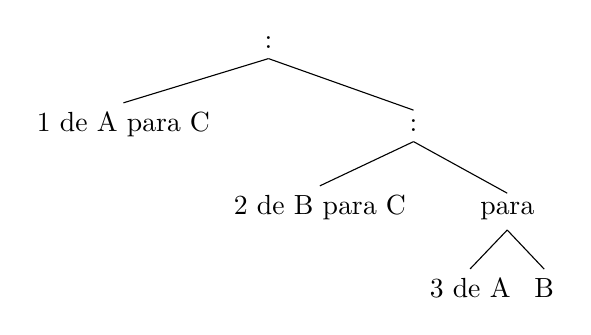
\begin{tikzpicture}
          \Tree 	[.{:}
                        [.{1 de A para C}
                        ]
                        [.{:}
                            [.{2 de B para C}
                            ]
                            [.{para}
                                [.{3 de A}
                                ]
                                [.{B}
                                ]
                            ]
                        ]
                    ]
    \end{tikzpicture}
\end{center}
\begin{center}
    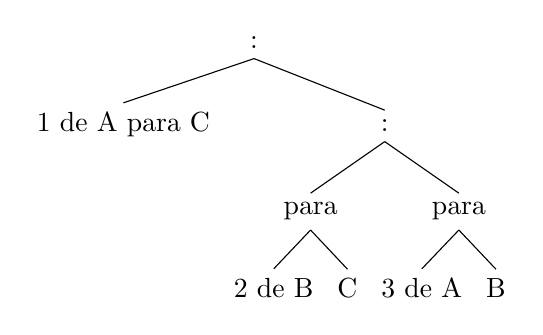
\begin{tikzpicture}
          \Tree 	[.{:}
                        [.{1 de A para C}
                        ]
                        [.{:}
                            [.{para}
                                [.{2 de B}
                                ]
                                [.{C}
                                ]
                            ]
                            [.{para}
                                [.{3 de A}
                                ]
                                [.{B}
                                ]
                            ]
                        ]
                    ]
    \end{tikzpicture}
\end{center}
\begin{center}
    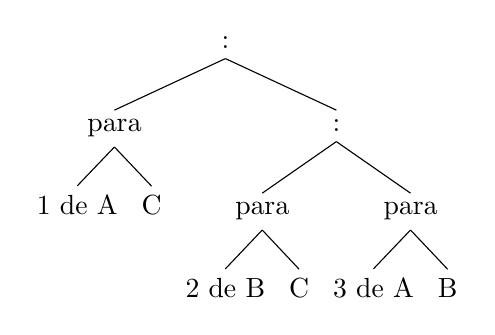
\begin{tikzpicture}
          \Tree 	[.{:}
                        [.{para}
                            [.{1 de A}
                            ]
                            [.{C}
                            ]
                        ]
                        [.{:}
                            [.{para}
                                [.{2 de B}
                                ]
                                [.{C}
                                ]
                            ]
                            [.{para}
                                [.{3 de A}
                                ]
                                [.{B}
                                ]
                            ]
                        ]
                    ]
    \end{tikzpicture}
\end{center}
\begin{center}
    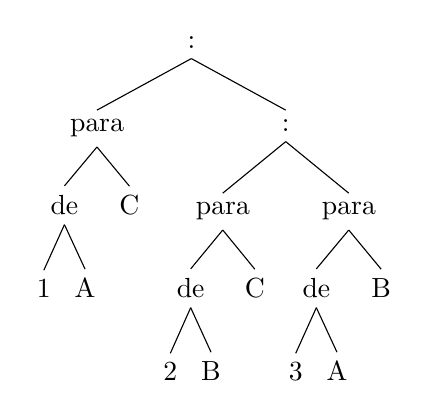
\begin{tikzpicture}
          \Tree 	[.{:}
                        [.{para}
                            [.{de}
                                [.{1}
                                ]
                                [.{A}
                                ]
                            ]
                            [.{C}
                            ]
                        ]
                        [.{:}
                            [.{para}
                                [.{de}
                                    [.{2}
                                    ]
                                    [.{B}
                                    ]
                                ]
                                [.{C}
                                ]
                            ]
                            [.{para}
                                [.{de}
                                    [.{3}
                                    ]
                                    [.{A}
                                    ]
                                ]
                                [.{B}
                                ]
                            ]
                        ]
                    ]
    \end{tikzpicture}
\end{center}

\end{document}